\documentclass{beamer}

\usetheme{CambridgeUS}
\usecolortheme{orchid}

\usepackage{graphicx}
\usepackage{tikz}
\usepackage{listings}
\usepackage{colortbl}

\tikzstyle{block} = [rectangle, draw, text width=4.5em, text centered, minimum height=2em]
\lstset{basicstyle=\small\ttfamily}



\lstset{
  language=Java,
  basicstyle=\ttfamily\small,
  keywordstyle=\color{blue},
  commentstyle=\color{green!60!black},
  stringstyle=\color{red},
  showstringspaces=false,
  breaklines=true
}

\setbeamertemplate{navigation symbols}{} % Remove navigation symbols

\title{API Design and Management}
\author{Mohamed Sweelam}
\institute{Software Engineer}
\date{}

% Add the title graphic here
\titlegraphic{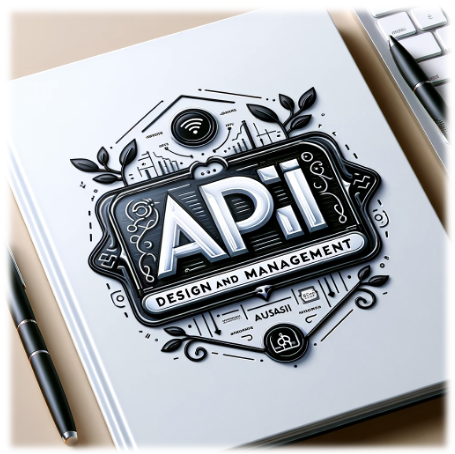
\includegraphics[width=7cm, height=3.5cm]{img/course-logo.png}}

\begin{document}

\begin{frame}
  \titlepage
\end{frame}

\begin{frame}{Outline}
  \tableofcontents
\end{frame}

\section{Course Objectives}
\begin{frame}
	\frametitle{Objectives} % Table of contents slide, comment this block out to remove it
		\begin{enumerate}
			\item<1-> {Provide good Arabic content for the topic}
			\item<2-> {Overview of API Design and Management}
			\item<3-> {Role and Importance of APIs in Distributed Systems}
			\item<4-> {The best practices you should follow today}
		\end{enumerate}
\end{frame}

\section{Understanding APIs}
\begin{frame}{Understanding APIs}
	\begin{block}{Definition \tiny{\textit{wikipedia}}}
		\small{ Application programming interface (API) is a way for two or more computer programs or components to communicate with each other. It is a type of software interface, offering a service to other pieces of software.}
	\end{block}
	
	\begin{block}{Definition \tiny{\textit{ChatGPT}}}
		\small{ API (Application Programming Interface) is a set of rules, protocols, and tools for building software applications. It specifies how software components should interact and is used to enable the integration between different software systems. }
	\end{block}
	
	\begin{alertblock}{History \tiny{\textit{wikipedia}}}
		\small{ The term "application program interface" is first recorded in a paper called Data structures and techniques for remote computer graphics in 1968. The authors use the term to describe the interaction of an application "Graphics Program" with the rest of the computer system. }
	\end{alertblock}
  
\end{frame}

\begin{frame}{Understanding APIs \small{\textit{(OSI Model)}}}
	\begin{center}
    		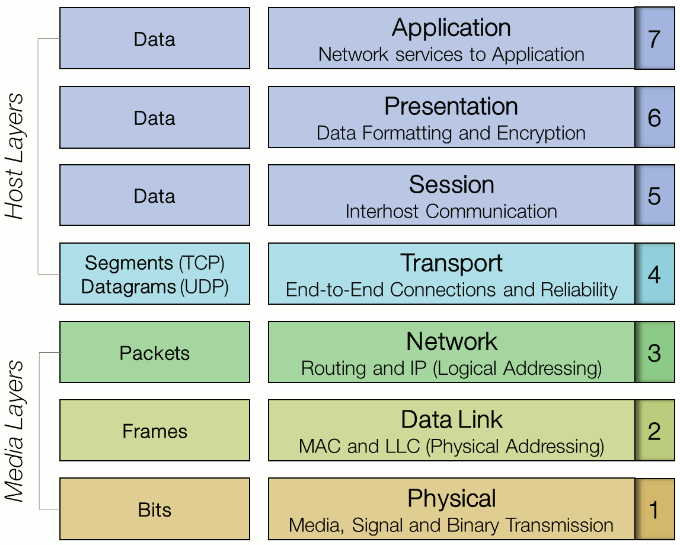
\includegraphics[width=0.8\textwidth, height=0.7\textheight]{img/osi-model.png}
  \end{center}
  
  \tiny { source:\href{https://www.coengoedegebure.com/osi-model}{\textcolor{blue}{coengoedegebure.com/osi-model}}}
\end{frame}

\begin{frame}{Understanding APIs}
	\begin{center}
    		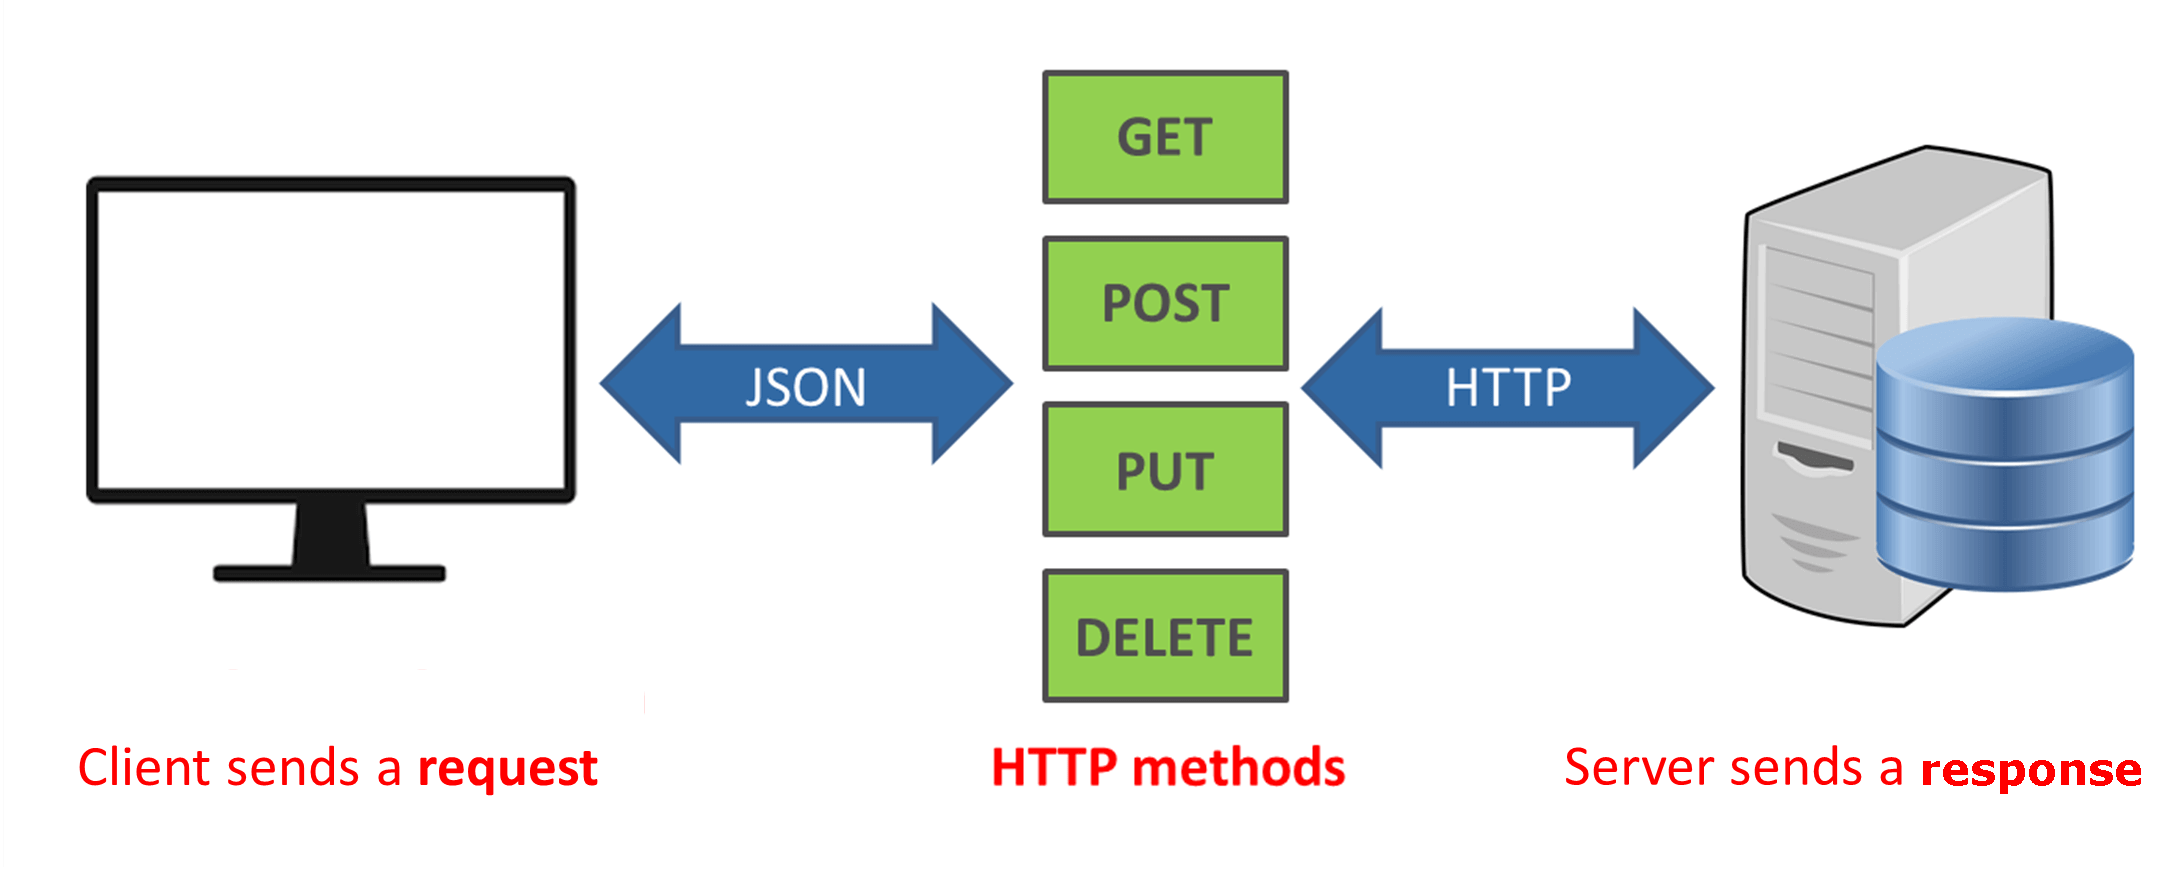
\includegraphics[width=0.6\textwidth, height=0.4\textheight]{img/api-client-to-server.png}
  \end{center}
  
  \tiny { source:\href{https://phpenthusiast.com/blog/what-is-rest-api}{\textcolor{blue}{phpenthusiast.com/blog/what-is-rest-api}}}
\end{frame}
 
\section{API Design Principles}
\begin{frame}{API Design Principles}
  \begin{itemize}
    \item Fundamentals of Good API Design
    \item Designing for Scalability and Performance
    \item API Versioning Strategies
  \end{itemize}
\end{frame}

\section{RESTful API Design}
\begin{frame}{RESTful API Design}
  \begin{itemize}
    \item RESTful Architecture Principles
    \item Designing RESTful Services (Endpoints, HTTP Methods, Status Codes)
    \item Best Practices in RESTful API
  \end{itemize}
\end{frame}



\section{Advanced API Protocols}
\begin{frame}{Advanced API Protocols}
  \begin{itemize}
    \item Introduction to GraphQL and Its Advantages
    \item Implementing gRPC for Microservices
    \item Comparison of Different API Styles
  \end{itemize}
\end{frame}

\section{API Documentation and Specification}
\begin{frame}{API Documentation and Specification}
  \begin{itemize}
    \item Importance of Comprehensive API Documentation
    \item Tools for API Documentation (Swagger, OpenAPI Specification)
    \item Maintaining and Versioning API Documentation
  \end{itemize}
\end{frame}

\section{API Security}
\begin{frame}{API Security}
  \begin{itemize}
    \item Authentication and Authorization Mechanisms (OAuth, JWT)
    \item Securing API Endpoints
    \item Handling Sensitive Data and Privacy Concerns
  \end{itemize}
\end{frame}

\section{API Testing and Quality Assurance}
\begin{frame}{API Testing and Quality Assurance}
  \begin{itemize}
    \item Writing Effective API Tests
    \item Tools and Frameworks for API Testing
    \item Performance Testing and Load Testing for APIs
  \end{itemize}
\end{frame}


\section{API Management and Lifecycle}
\begin{frame}{API Management and Lifecycle}
  \begin{itemize}
    \item The Lifecycle of API Development
    \item API Deployment Strategies
    \item Monitoring and Analytics for APIs
  \end{itemize}
\end{frame}

\section{Conclusion}
\begin{frame}{Conclusion}
  \begin{itemize}
    \item Recap of Key Learnings
    \item Emerging Trends in API Development
  \end{itemize}
\end{frame}

\end{document}
